\documentclass[a4paper,11pt]{article}
    \usepackage[utf8]{inputenc}
    \usepackage[italian]{babel}
    \usepackage[maxbibnames=99,backend=bibtex]{biblatex}
    \usepackage{hyperref}
    \usepackage{listings}
    \usepackage{color}
    \usepackage{graphicx}
    \usepackage{titling}
    
    \addbibresource{ref.bib}
    \graphicspath{ {images/} }
    \lstset{frame=tb,
        language=C++,
        breaklines=true,
        showstringspaces=false,
        columns=flexible,
        numbers=none,
        commentstyle=\color{dkgreen},
        stringstyle=\color{mauve},
        tabsize=3
    }
    % define the title
    \author{
        Tirocinante: Coccomini Davide \\
        Tutor universitario: Pistolesi Francesco, Lazzerini Beatrice \\
        Tutor aziendale: Maccari Antonio, Maccari Francesca
    }


    %define logo
    \pretitle{%
    \begin{center}
        \LARGE
        
\includegraphics[scale=0.6]{logo}\\[\bigskipamount]
    }
    \posttitle{\end{center}}
    %\pagestyle{headings}
    \title{\textbf{UNIVERSITA DEGLI STUDI DI PISA} \\[0.4in]
        Relazione Finale Tirocinio \\
    Scuola di Ingegneria \\
    Dipartimento di Ingegneria dell’Informazione \\[1in]
    Influenza del numero di lunghezze d’onda sulla qualità dell’immagine spettrale.}
    \date{}
    
    
    \definecolor{mygreen}{rgb}{0,0.6,0}
    
    \lstset{  
        numbers=left,
        numbersep=5pt,
        commentstyle=\color{mygreen},
        keywordstyle=\color{blue}\ttfamily,
        stringstyle=\color{red}\ttfamily  
    }
    
    
    %link cliccabili
    \hypersetup{colorlinks=true, linktoc=all,  linkcolor=black,citecolor=black}
    \newpage
    \begin{document}

    \maketitle  
    \newpage
       % insert the table of contents
        \tableofcontents
        \newpage
        \section{Introduzione}
        \subsection{Lo spettro visibile}
        Lo “spettro del visibile” si trova nella parte centrale dello spettro ottico, il quale
        comprende anche i raggi infrarossi e quelli ultravioletti. E’ composto da quella parte di
        spettro elettromagnetico che include tutte le colorazioni percepite dall’occhio umano,
        partendo dal rosso fino ad arrivare al viola.
        \begin{figure}[h]
            \centering
            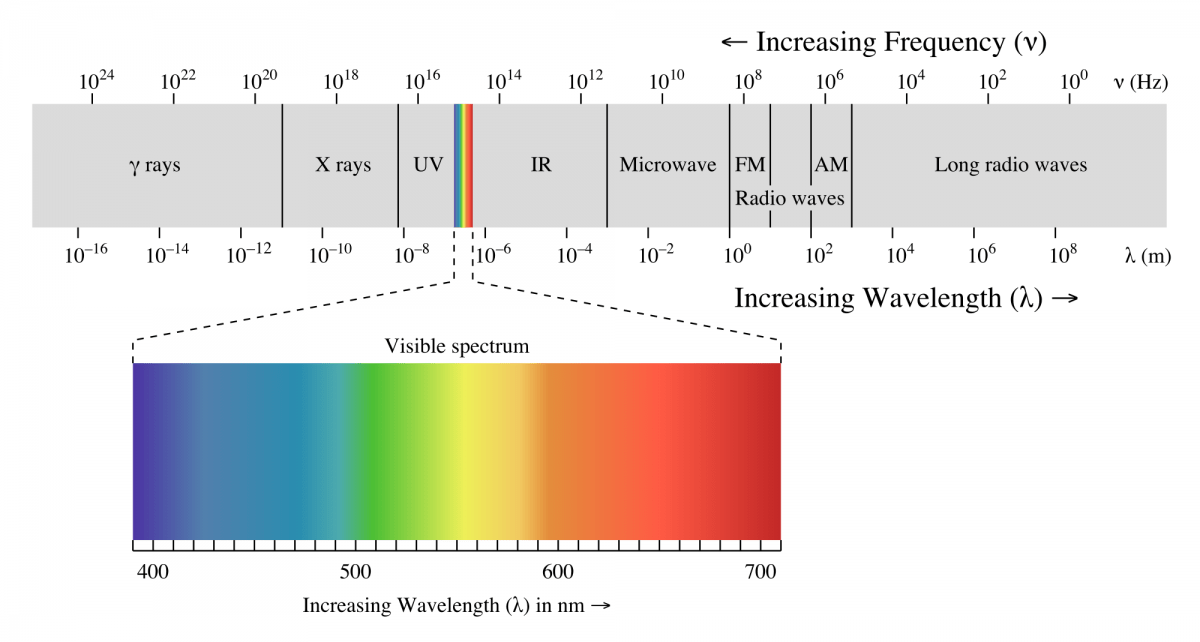
\includegraphics[scale=0.3]{colorimetria3}
            \caption{"Lo spettro visibile"}
        \end{figure}
        \newpage
        \subsection{Percezione del colore}
        Il colore nasce dalla luce. La luce che colpisce un oggetto viene parzialmente assorbita a
        seconda del colore. La parte non assorbita viene riflessa e trasmessa ai recettori cromatici
        all’interno dell’occhio umano. Questi ultimi trasformano la luce assorbita in impulsi che
        percorrono le vie nervose fino a raggiungere il cervello, dove vengono interpretati: nasce così
        un’impressione cromatica. Dal punto di vista prettamente biologico il colore si genera pertanto
        nell’occhio dell’osservatore e costituisce un’impressione sensoriale.

        A proposito di impressione sensoriale: ciascun individuo "percepisce" il colore in modo
        differente. Tale fenomeno non è riconducibile solamente al fatto che non esistono mai due occhi
        uguali tra loro. Anche l’interpretazione del colore varia infatti da individuo ad individuo.
        Perfino la stessa persona può percepire differentemente il colore in momenti diversi ed in base
        allo stato d’animo. Il colore stesso può pertanto generare sensazioni differenti. 

        \begin{figure}[h]
            \centering
            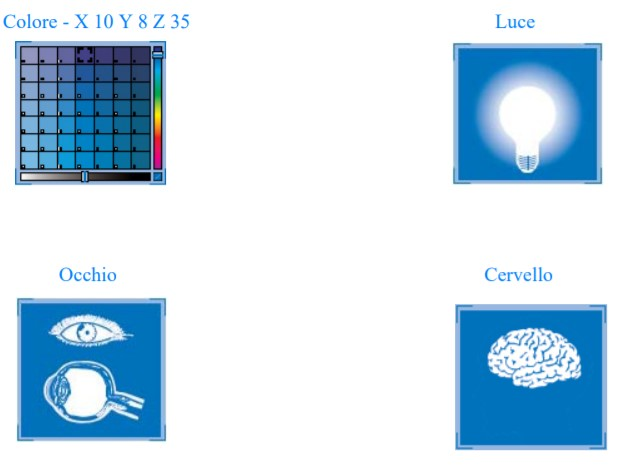
\includegraphics[scale=0.8]{colorimetria1}
            \caption{"Percezione del colore"}
        \end{figure}
        \newpage
        \subsection{Metamerismo}
        Ciascuno di noi conosce il fenomeno per cui un oggetto colorato osservato sotto una
        determinata sorgente di luce come la luce diurna, presenta un colore diverso da quello visto
        sotto un altra sorgente come ad esempio la luce di una lampadina ad incandescenza. Tale
        mutamento cromatico, caratteristico di quasi tutti gli oggetti colorati, viene spesso erroneamente
        definito metamerismo. Ma che cos’è in realtà il metamerismo?
        Il metamerismo può essere spiegato in termini di variazioni dei valori di tristimolo (X,Y e Z),
        che quantificano la percezione del colore. Due campioni sono uguali sotto una determinata
        sorgente di luce quando i relativi valori XYZ sono identici per quel particolare illuminante. Tale
        condizione è sempre soddisfatta sotto tutti gli illuminanti nel caso di campioni identici
        caratterizzati da curve di riflettanza uguali. I campioni metamerici presentano invece curve di
        riflettanza diverse. Ne consegue che tali campioni possono avere valori di tristimolo XYZ
        uguali sotto un certo illuminante ed apparire uguali, ma al mutare dell' illuminante, valori XYZ
        diversi ed apparire dunque diversi fra loro. 
        
        \begin{figure}[h]
        \centering
        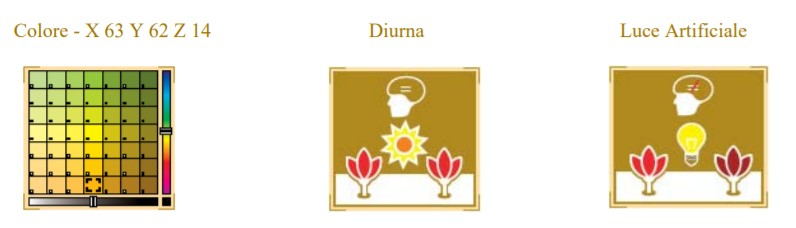
\includegraphics[scale=0.8]{colorimetria2}
        \caption{"Metamerismo"}
        \end{figure}
        
        \newpage

        \subsection{Scanner spettrofotometrico}
        Lo scanner spettrofotometrico è nato per riprendere immagini adatte a
        costituire archivi di dipinti e di altre opere d’arte di superficie piana, utilizzabili per scopi di diagnostica, di
        restauro e di multimedialità. Le immagini d’archivio devono possedere almeno questi requisiti: riprodurre
        fedelmente il colore, essere confrontabili con immagini dello stesso oggetto riprese a distanza di tempo,
        essere stabili nel tempo per fornire una documentazione storica delle opere d’arte. Immagini di questo tipo si
        ottengono se sono basate sulla misurazione del fattore di riflessione spettrale della loro superficie. Esso è
        determinato dal rapporto tra il segnale dovuto alla luce riflessa dall’opera d’arte e quella riflessa da un
        riflettore ideale in identiche condizioni di misurazione ed è quindi indipendente dalle specifiche tecniche
        della strumentazione usata per la sua misurazione. Inoltre, consente di esprimere il colore nello spazio
        colorimetrico dell’Osservatore Standard della CIE che è equivalente allo spazio colorimetrico del sistema di
        visione dell’uomo. Le immagini basate sul fattore di riflessione spettrale costituiscono una nuova categoria di
        immagini digitali: le immagini spettrali.
        Le immagini spettrali hanno parecchi vantaggi rispetto alle immagini digitali tricromatiche perché consentono:
        \begin{enumerate} 
             \item di sfruttare al meglio il sensore elettronico (numero pixel-immagine uguale numero pixel-sensore);
             \item il controllo del metamerismo;
             \item la codifica dei colori in ogni spazio colorimetrico;
             \item il loro uso anche con i futuri sviluppi della colorimetria;
             \item la riproduzione su base spettrale;
             \item di scegliere l’illuminante e il tipo di Osservatore Standard CIE per il calcolo del colore.
        \end{enumerate}
        Lo scanner iperspettrale ottiene informazioni relative alla luce riflessa dall'immagine ottenendo così una serie di immagini su più frequenze che unite compongono l'immagine vera e propria.
    
    \newpage
    
        \begin{figure}[h]
            \centering
            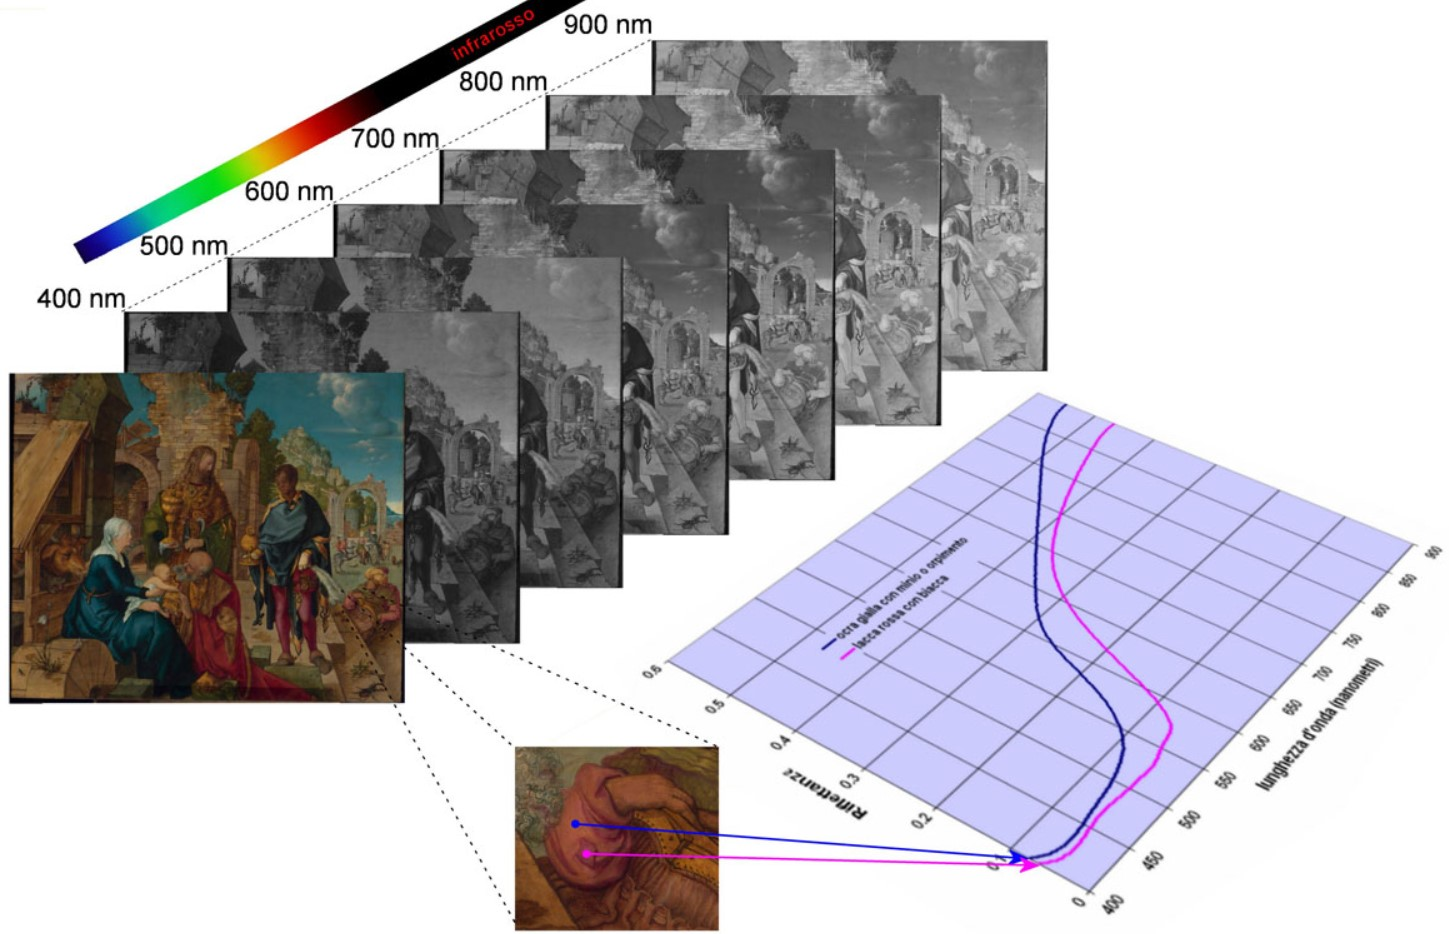
\includegraphics[scale=0.4]{colorimetria4}
            \caption{"Risoluzione"}
        \end{figure}

    \newpage
    \section {Obiettivo del tirocinio}
    \subsection{Confronto tra immagini}
    Il tirocinio ha l’obiettivo di ricercare una metodologia che misuri la differenza esistente tra due immagini aventi il medesimo soggetto, ma realizzate in tempi o con mezzi differenti affinché si possa 
    capire qual è il minimo numero di bande che uno scanner deve ottenere continuando ad ottenere un risultato soddisfacente.
    Riducendo le bande è possibile ottimizzare i processi produttivi, abbattendo i tempi di acquisizione e produzione.
    Nel dettaglio, lo scanner estrae immagini su 31 bande differenti ottenendo come risultato un'immagine estremamente fedele all'originale. Si cercherà di confrontare questa immagine con una ottenuta sullo stesso soggetto ma con sole 21 bande. 
    
    \newpage
    
    \subsubsection{SSIM}
    Risulta quindi necessario individuare un metodo oggettivo per il confronto tra l'immagine originale e quella compressa. 
    Si è deciso di utilizzare lo structural similarity index method (SSIM) che è un metodo ampiamente utilizzato per la predizione la qualità percettiva delle immagini televisive e cinematografiche.
    L'SSIM considera il degrado dell'immagine come cambiamento percepito nelle informazioni strutturali, mentre incorpora anche importanti fenomeni percettivi, inclusi sia il mascheramento della luminanza che i termini di mascheramento del contrasto. 
    \subsubsection{Algoritmo}
    L'indice SSIM viene calcolato su varie finestre di un'immagine. La misura tra due finestre $x$ e $y$ di dimensione NxN è: \\[0.2in]
        $$\hbox{SSIM}(x,y) = \frac{(2\mu_x\mu_y + c_1)(2\sigma_{xy} + c_2)}{(\mu_x^2 + \mu_y^2 + c_1)(\sigma_x^2 + \sigma_y^2 + c_2)}$$
    \begin{enumerate} 
        \item $\mu_x$ la media di $x$;
        \item $\mu_y$ la media di $y$;
        \item $\sigma_x^2$ la varianza di $x$;
        \item $\sigma_y^2$ la varianza di $y$;
        \item $\sigma_xy$ la covarianza di $x$ e $y$;
        \item $c_1=(k_1L)^2$, $c_2=(k_2L)^2$ due variabili per stabilizzare la divisione con il denominatore inadatto;
        \item $L$ la gamma dinamica dei valori dei pixel;
        \item $k_1=0.01$ e $k_2=0.03$ predefiniti.
   \end{enumerate}

   \newpage

    \subsubsection{Componenti della formula}
    La formula SSIM si basa su tre misurazioni di confronto tra i campioni di $x$ e $y$: luminanza $l$, contrasto $c$ e struttura $S$. Le singole funzioni di confronto sono:
    \begin{enumerate} 
        \item $l(x,y)=\frac{2\mu_x\mu_y + c_1}{\mu^2_x + \mu^2_y + c_1}$
        \item $c(x,y)=\frac{2\sigma_x\sigma_y + c_2}{\sigma^2_x + \sigma^2_y + c_2}$
        \item $s(x,y)=\frac{\sigma_{xy} + c_3}{\sigma_x \sigma_y + c_3}$
    \end{enumerate}
    con, oltre alle definizioni di cui sopra:\\
    $c_3 = c_2 / 2$ 

    L'SSIM è quindi una combinazione ponderata di tali misure comparative:
    $$SSIM(x,y) = [l(x,y)^\alpha \cdot c(x,y)^\beta \cdot s(x,y)^\gamma$$
    
    \newpage

    \section{Svolgimento}

    \subsection{Strumenti}
    Per affrontare i problemi relativi alla manipolazione delle immagini si è deciso di utilizzare il linguaggio C++ con il supporto della libreria OpenCV.
    OpenCV è una nota libreria open-source disponibile in C++, Python e Java e permette di effettuare le operazioni più disparate sulle immagini.
    Inoltre, essa include a sua volta altre librerie come la libtiff che utilizzeremo per la lettura delle immagini.
    
    \subsubsection{Tavola Savoia-Navona-Matte}
    Come soggetto dell'immagine è stata scelta la tavola Savoia-Navona-Matte, rappresentative di numerose sfumature di colore ed utilizzare per effettuare test sugli spettrofotometri.

    \begin{figure}[h]
        \centering
        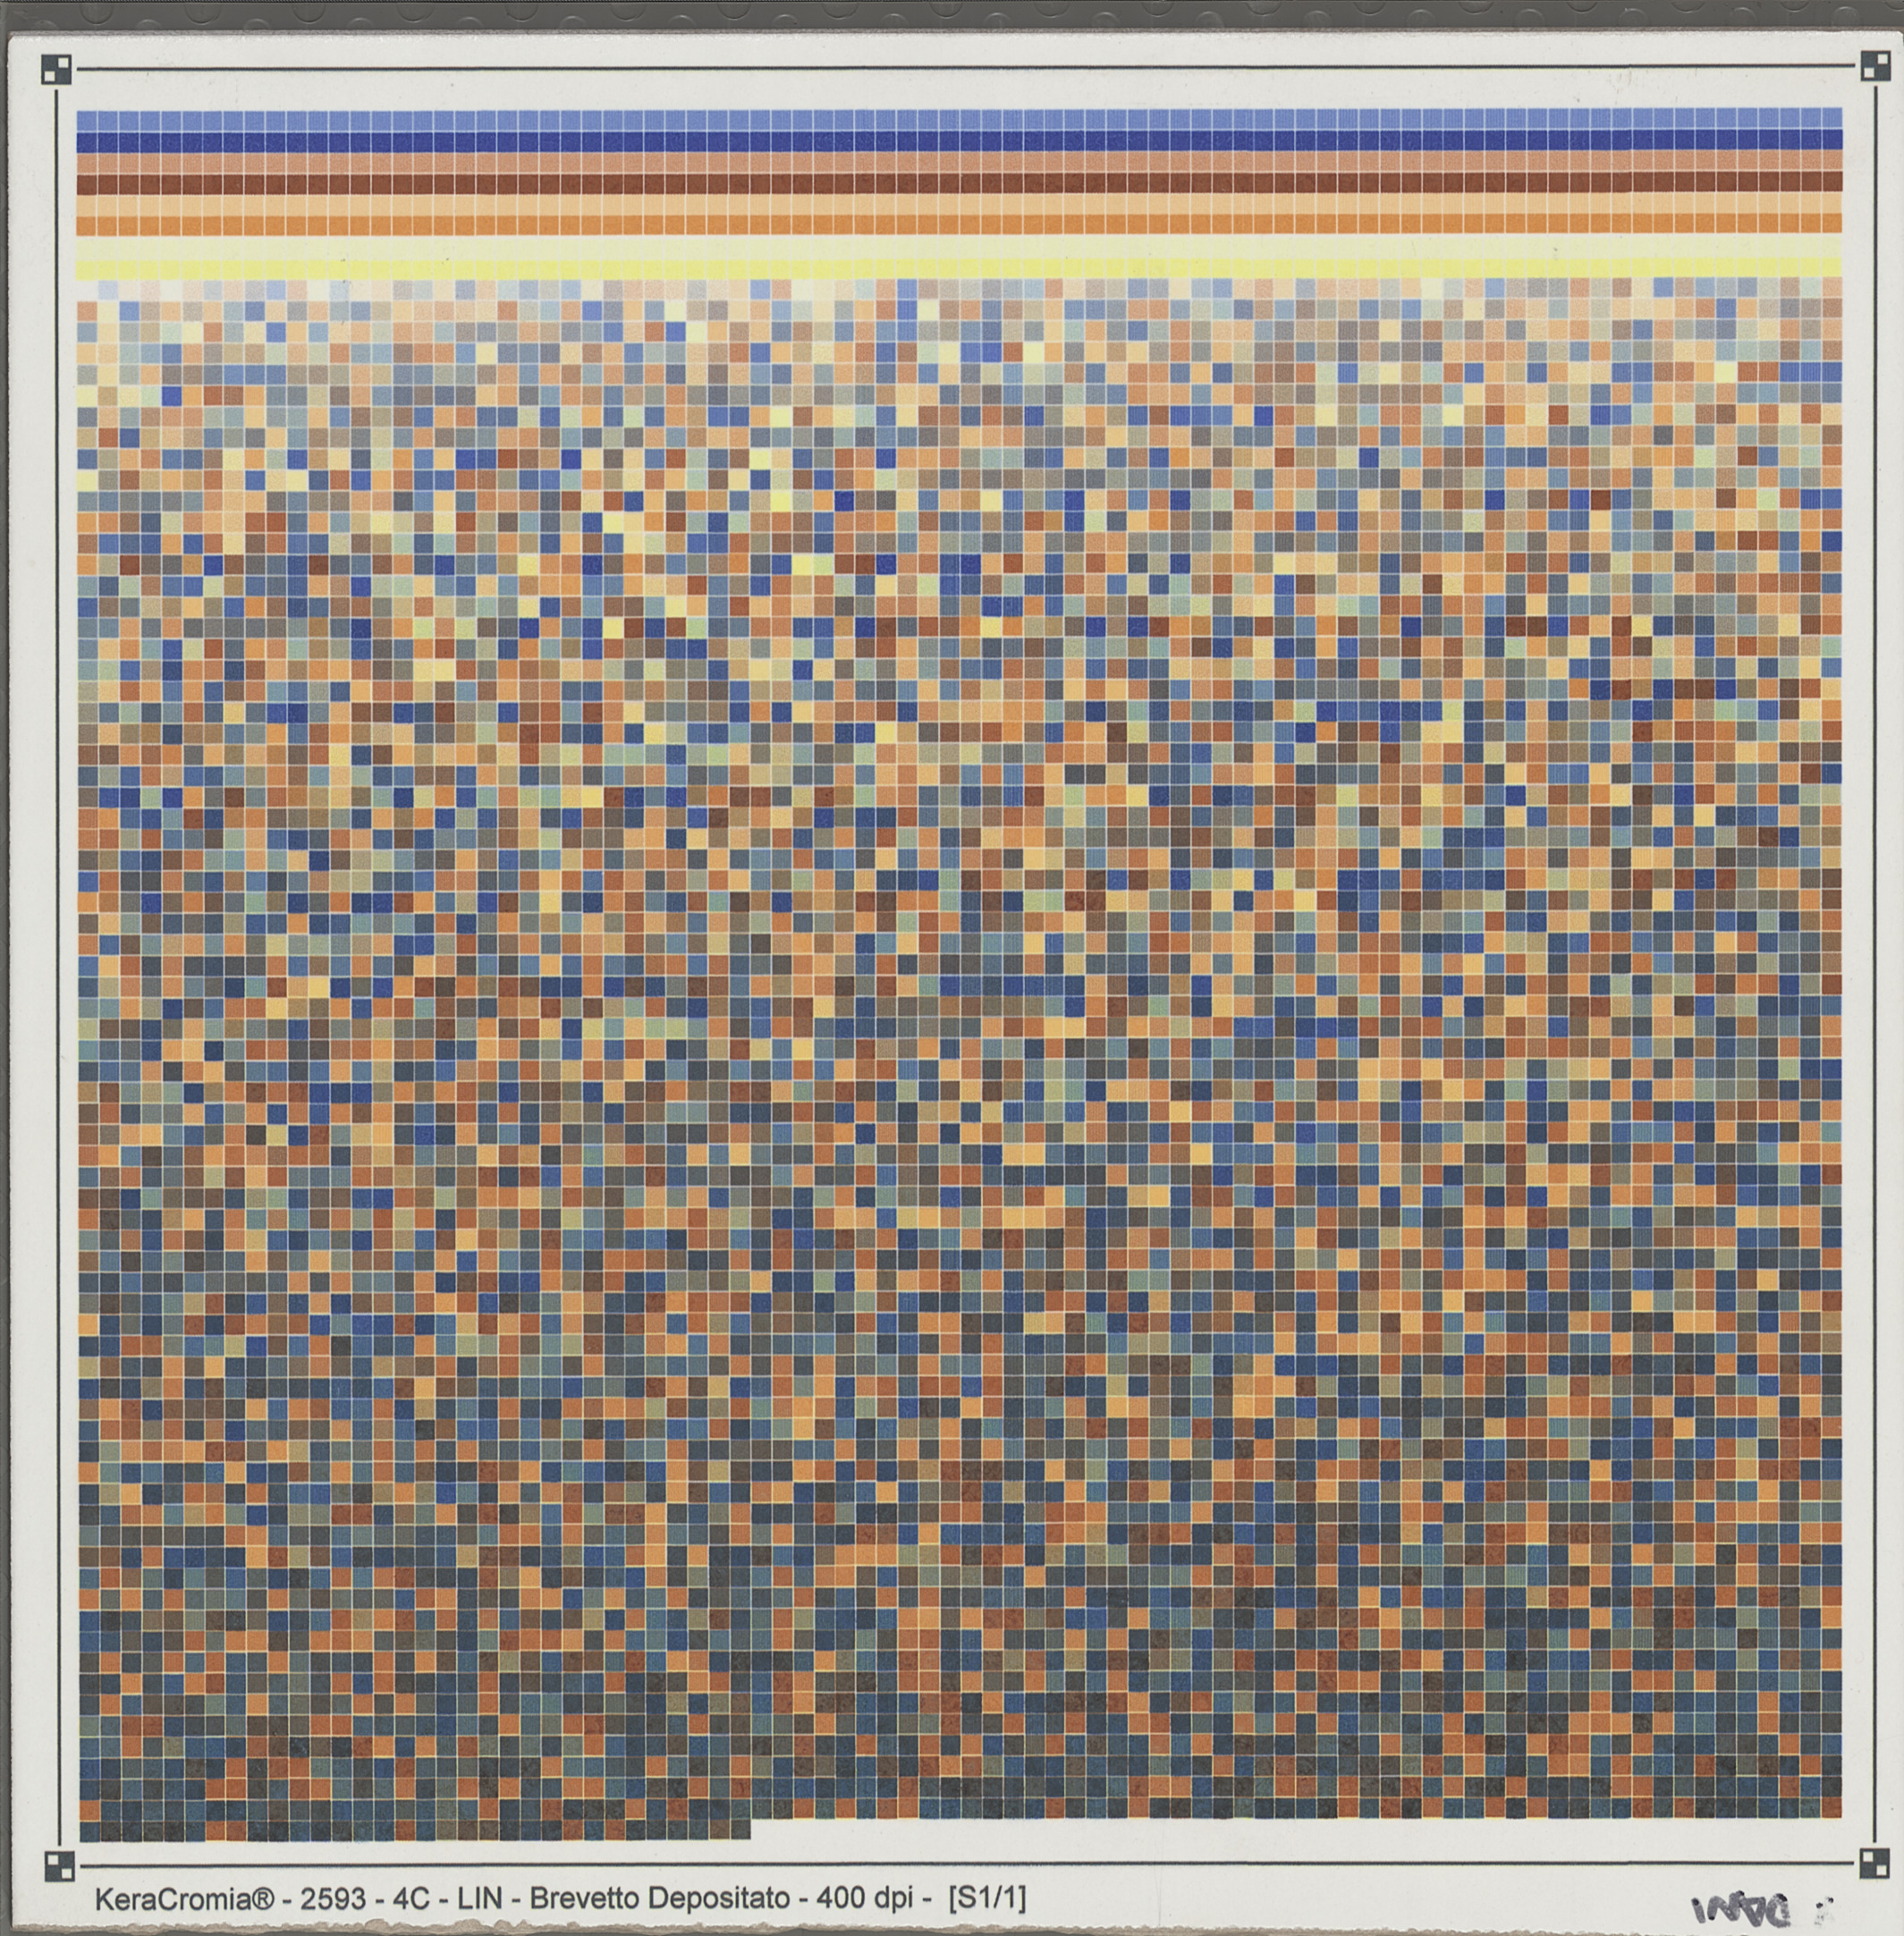
\includegraphics[scale=0.4]{tavola}
        \caption{"Tavola Savoia-Navona-Matte"}
    \end{figure}

    La tavola è ottenuta come il risultato dell'unione di 31 bande nello spettro visibile da 400nm a 700nm, una ogni 10nm.
    In Figura 6 sono rappresentati alcuni esempi significativi delle bande sopracitate.
    \begin{figure}[h]
        \centering
        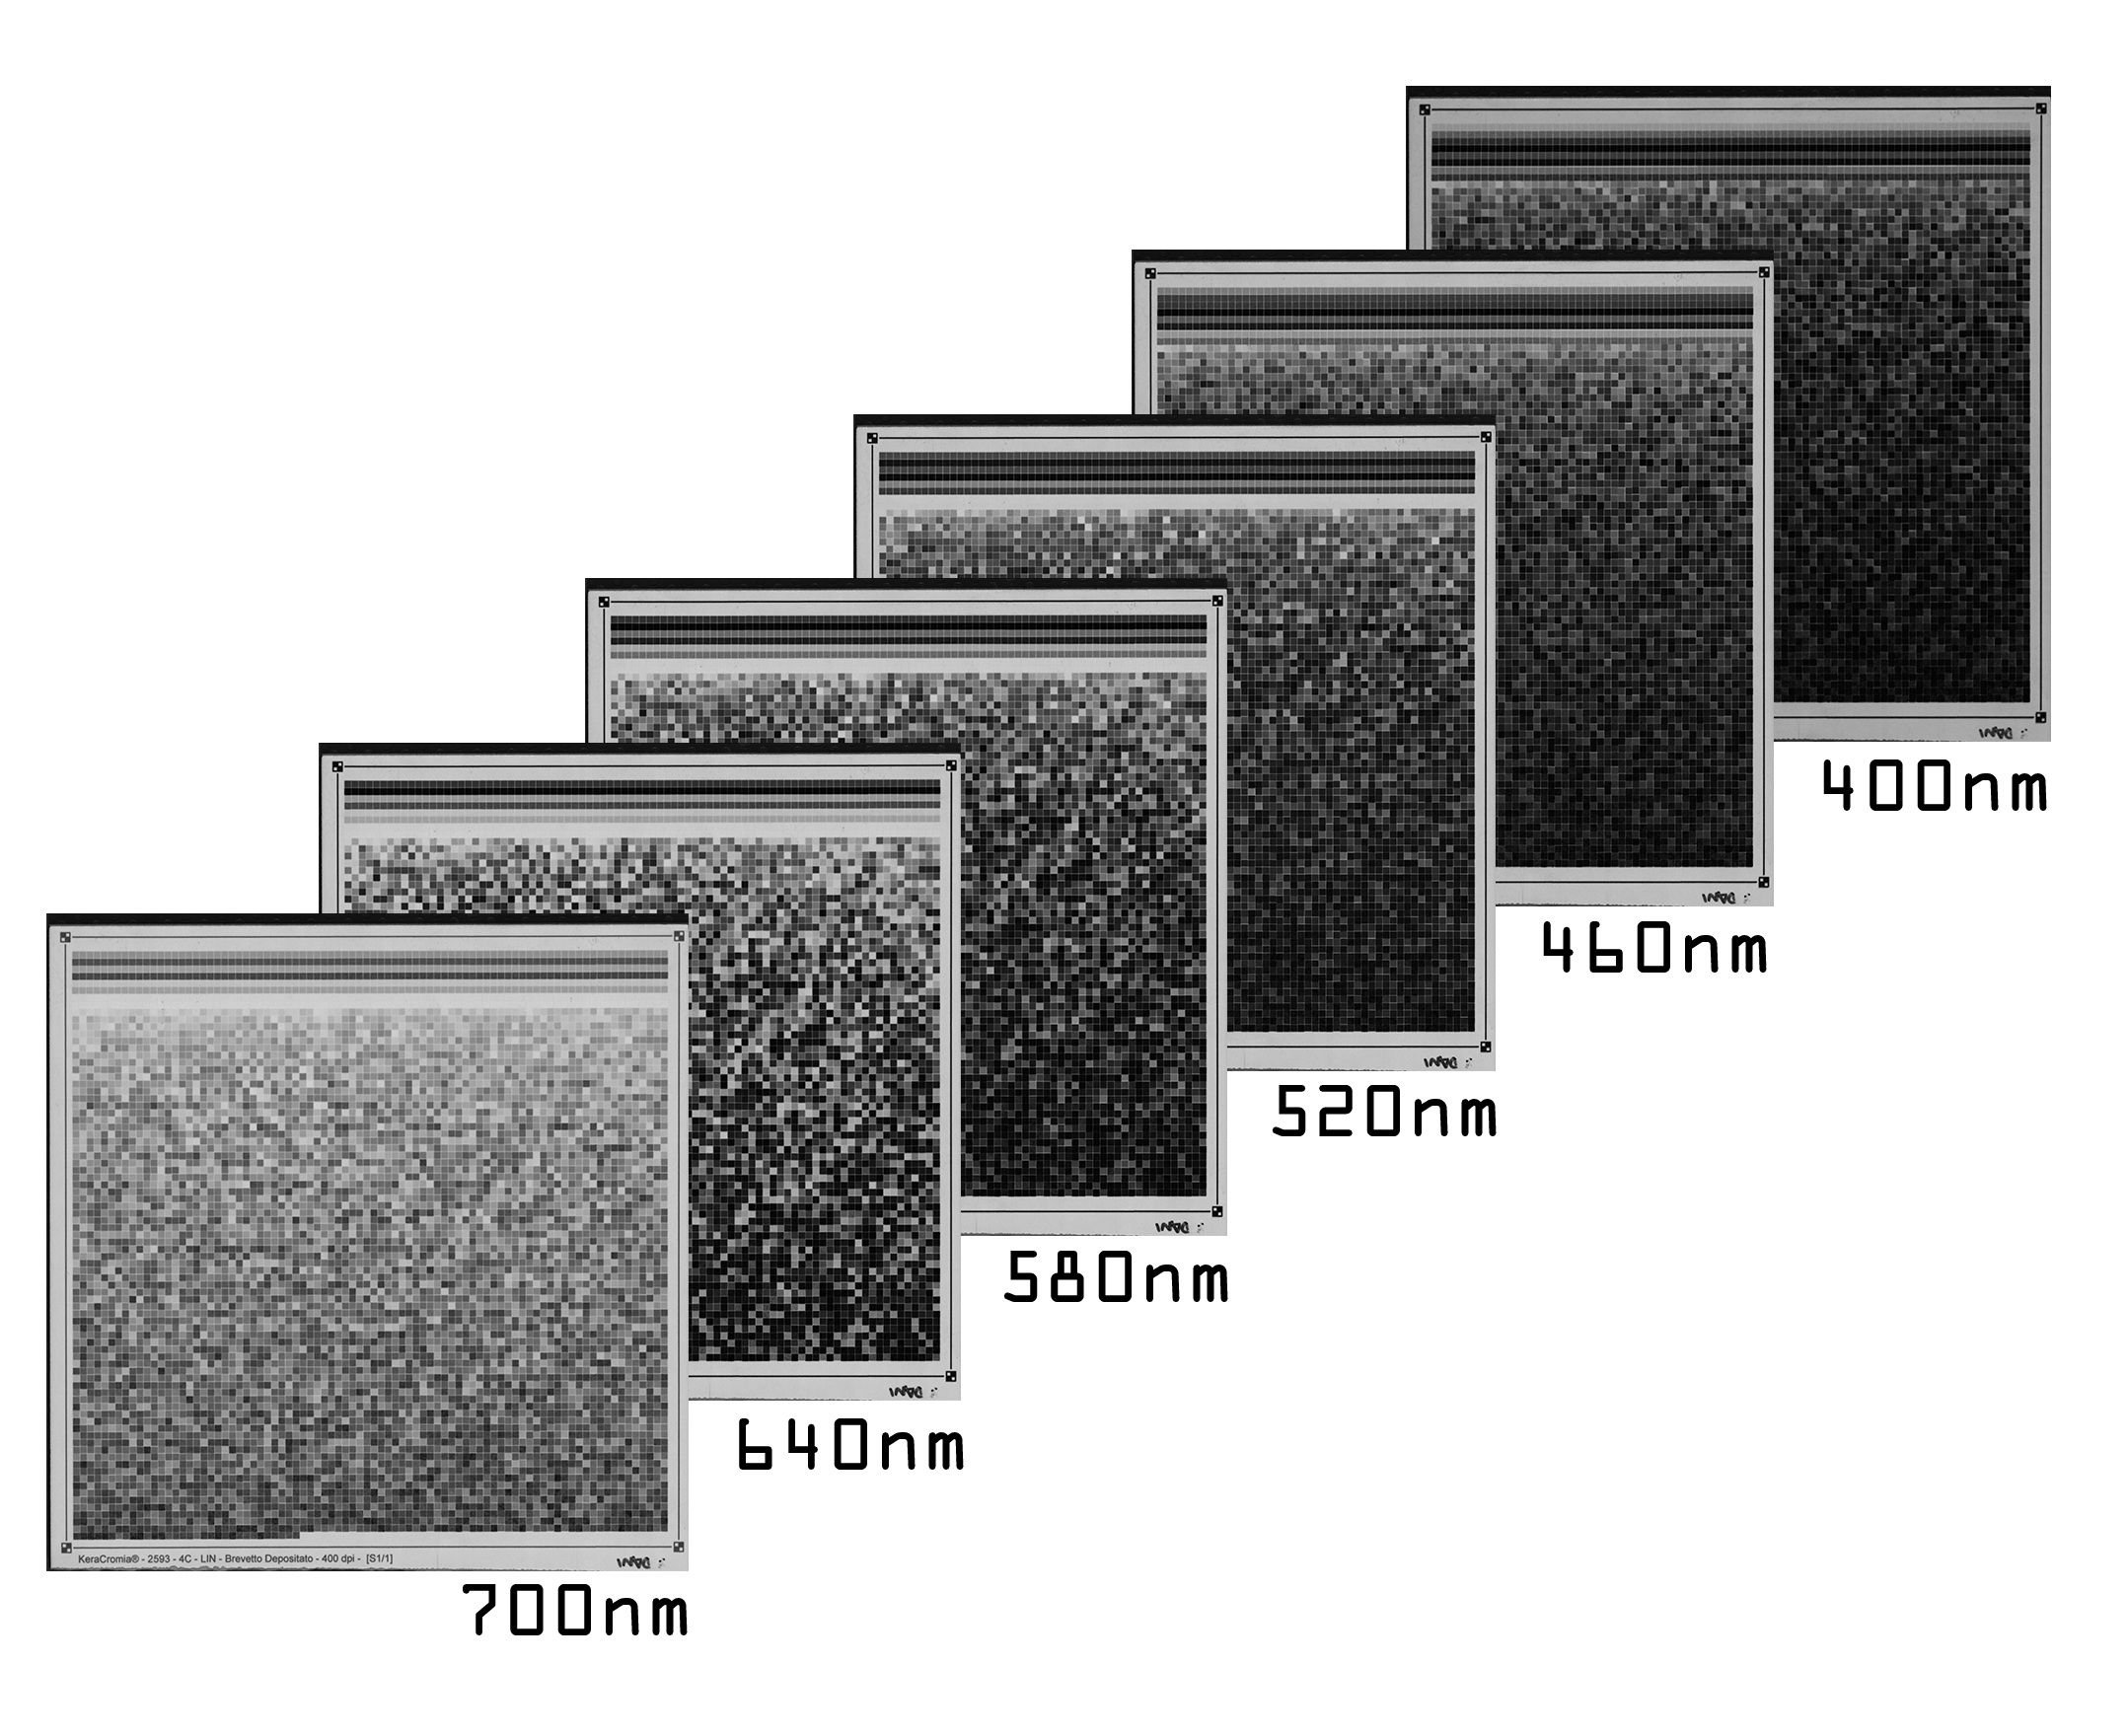
\includegraphics[scale=0.15]{tavola2}
        \caption{"Suddivisione in bande della tavola Savoia-Navona-Matte"}
    \end{figure}


    \newpage
    \subsection{Rappresentazione delle immagini}
    Avendo a disposizione due immagini in formato TIFF, il primo problema da affrontare è riuscire a rappresentare questa immagine in una struttura dati che possa essere poi manipolata per ottenerne informazioni.
    Per fare ciò sfruttiamo la libreria OpenCV e, in particolare, la libtiff. Tramite le funzioni di questa libreria, si legge l'immagine e la si trasforma in una matrice sfruttando la struttura dati "Mat" messa a disposizione dalla OpenCV:
 
    \begin{lstlisting}[language=C++]
            bool tifToMat(Mat& image,string imageName){
                // Read images and create the Mat
                TIFF* tif = TIFFOpen(imageName.c_str(), "r");
                
                if (tif) {
                    do {
                        unsigned int width, height;
                        uint32* raster;

                        // Get the size of the tiff
                        TIFFGetField(tif, TIFFTAG_IMAGEWIDTH, &width);
                        TIFFGetField(tif, TIFFTAG_IMAGELENGTH, &height);

                        uint npixels = width*height; // Get the total number of pixels

                        raster = (uint32*)_TIFFmalloc(npixels * sizeof(uint32)); // Allocate temp memory (bitmap)
                        if (raster == NULL) // Check the raster's memory was allocated
                        {
                            TIFFClose(tif);
                            cerr << "Raster allocate error" << endl;
                            return false;
                        }
                                
                        // Check the tif read to the raster correctly
                        if (!TIFFReadRGBAImage(tif, width, height, raster, 0))
                        {
                            TIFFClose(tif);
                            cerr << "Raster read error" << endl;
                            return false;
                        }

                        // Create a new matrix of width x height with 8 bits per channel and 4 channels (RGBA)
                        image = Mat(width, height, CV_8UC4); 
                                
                        // Itterate through all the pixels of the tif
                        for (uint x = 0; x < width; x++)
                            for (uint y = 0; y < height; y++)
                            {
                                uint32& TiffPixel = raster[y*width+x]; // Read the current pixel of the TIF
                                Vec4b& pixel = image.at<Vec4b>(Point(y, x)); // Read the current pixel of the matrix
                                pixel[0] = TIFFGetB(TiffPixel); // Set the pixel values as BGRA
                                pixel[1] = TIFFGetG(TiffPixel);
                                pixel[2] = TIFFGetR(TiffPixel);
                                pixel[3] = TIFFGetA(TiffPixel);
                            }
                        
                        // Free temp memory
                        _TIFFfree(raster); 

                        // Rotate the image 90 degrees 
                        image = image.t(); // Traspose
                        flip(image, image, 0);
                    
                    } while (TIFFReadDirectory(tif)); // Get the next tif to go into the channels

                TIFFClose(tif); // Close the tif file
                }else return false;
         return true;
        }
    \end{lstlisting}

    \newpage

    \subsection{Estrazione dell'indice}
    Adesso che le immagini sono state trasformate in strutture dati, è possibile ricavarne informazioni seguendo le formule precedentemente dette:
    \begin{lstlisting}[language=C++]
        double getSSIM(Mat & img_src, Mat & img_compressed, int block_size, bool show_progress = true)
        {
        double ssim = 0;

        if(img_src.cols != img_compressed.cols || img_src.rows != img_compressed.rows){
        cout<<"The images got different size"<<endl;
        return -1;
        }
        int nbBlockPerHeight = img_src.rows / block_size;
        int nbBlockPerWidth = img_src.cols / block_size;
            // Foreach block in the images
            for (int k = 0; k < nbBlockPerHeight; k++)
            {
                for (int l = 0; l < nbBlockPerWidth; l++)
                {
                    int m = k * block_size;
                    int n = l * block_size;

                    double avg_o 	= mean(img_src(Range(k, k + block_size), Range(l, l + block_size)))[0];
                    double avg_c 	= mean(img_compressed(Range(k, k + block_size), Range(l, l + block_size)))[0];
                    double sigma_o 	= variance(img_src, m, n, block_size);
                    double sigma_c 	= variance(img_compressed, m, n, block_size);
                    double sigma_co	= covariance(img_src, img_compressed, m, n, block_size);

                    ssim += ((2 * avg_o * avg_c + C1) * (2 * sigma_co + C2)) / ((avg_o * avg_o + avg_c * avg_c + C1) * (sigma_o * sigma_o + sigma_c * sigma_c + C2));
                    
                }
                // Progress %
                if (show_progress)
                    cout << "\r>>SSIM [" << (int) ((( (double)k) / nbBlockPerHeight) * 100) << "%]";
            }
                ssim /= nbBlockPerHeight * nbBlockPerWidth;

            if (show_progress)
            {
                cout << "\r>>SSIM [100%]" << endl;
                cout << "SSIM : " << ssim << endl;
            }
         return ssim;
        }
    \end{lstlisting}
    La funzione scorre come una finestra mobile (di dimensione block size) contemporaneamente l'immagine originale e quella compressa e ne calcola le varianze, le medie e la covarianza. 
    Ognuno di questi confronti contribuirà al risultato della funzione che sarà sempre un numero compreso tra -1 ed 1.
    Se le due immagini sono identiche, allora il risultato sarà 1 altrimenti sarà un numero sempre minore fino al -1 che rappresenta due immagini completamente diverse.
    
    \newpage
    
    \section{Conclusioni} 
    L'idea di utilizzare 21 bande anziché 31 ha generato un'immagine che, confrontata con l'originale, ha dato un indice SSIM di:
    +-X,XXXX
    Il risultato ci dice quindi che le immagini sono XXXXXXXX, segue quindi che XXXXX.
  
\end{document}